%Colle du Mercredi 28 a Janson, edp
\documentclass{scrartcl}

\usepackage{cmap}
\usepackage{lmodern}
\usepackage[T1]{fontenc}
\usepackage[french]{babel}
\usepackage{algorithm}
\usepackage{pdfpages}
\usepackage{algpseudocode}
\usepackage{ marvosym }
\usepackage{amsmath}
\usepackage{tikz}
\usepackage{amsfonts}
\usepackage{amssymb}

\title{Algorithmie // Homework 3 // Question 2}
\author{Oscar Garnier}
\date{\today}


\begin{document}
\newcommand{\E}[1]{\section*{Exo #1}}
\newcommand{\CR}[2]{\section*{#1 // note : #2}}
\newcommand{\Q}[1]{\section*{Exercise #1}}
\newcommand{\SQ}[1]{\subsection*{Question #1}}
\maketitle

\SQ{1}

Let us suppose by contradiction that there are two distinct minimum spanning trees in the graph, \( T_1, and T_2 \). 
Consider the set of all edges that are only in one of these two trees, we know it is non empty because the trees are distinct. 
Within this set, find the edge of lowest weight \( e_1 \). WLOG, we can suppose \( e_1 \in T_1 \). \( T_2 \cup e_1 \) contains a cycle, and at least one edge of this cycle is not in \( T_1 \) (or \( T-1 \) would contain a cycle), call this edge \( e_2 \). We know \( e_2 \in T_2 / T_1 \), which means \(w(e_2) > w(e_1 \). Since \( e_2 \) was part of a cycle in \( T_2 \cup e_1 \), \( T_2 \cup e_1 /e_2 \) is a still connected, hence it is a spanning tree (by cardinality), and it is of strictly lower weight. This is absurd.
The minimum spanning tree is unique. \\

The second-best minimum spaning tree is not thought; see attached document for an counter-example.

\SQ{2}

Let \( T \)  be the minimum spanning tree in \( G \). Let \( T' \) be some other tree that differs from \( T \) by more than one edge. Hence \( |T - T'| \geq 2 \). Choose \( p \in T - T'\) it's element of lowest weight.
Adding \( p \) to \( T' \) would cause a cycle, and there is an edge of this cycle in \( T' - T\) (or \( T \) would contain a cycle), let us call this edge \( q \in T' \).
Notice that, by construction, \( T' - q + p \) is a tree. \\

Suppose, by contradiction, \( w(q) < w(p) \). \\
If we were to add \( q \) to \( T \), we would get a cycle, and we know there is an element of \( T - T' \) in this cycle, call it \( p' \in T - T'\).
According to this construction, \( T - p' + q \) is a tree, so, by minimality of \( T \), \( w(q) > w(p') \).
This means \( w(p) > w(q) > w(p') \) which is contradictory with the minimality of \( p \) in \( T - T' \).\\
Hence, \( w(q) > w(p) \). But then \( T' - q + p \) is a tree of lower weight than \( T'\), yes distinct from \( T \), which means \( T' \) is not a second best spanning tree.


Hence, any second best spanning tree in \( G \) would differ from \( T \) by exactly one edge. Since we know such a tree exists (there are more that \( |V| - 1 \) edges, so more than 1 spanning tree), we know that there exists a second best spanning tree, differing from \( T \) by exactly one edge.


\SQ{3}

\begin{algorithm}
  \caption{Gte max weight in path}
  \label{oscar garnier}
  \begin{algorithmic}[1]

    \Function{FIND\_MAX\_PATH\_WEIGHTS}{$T, G$}
		\State Choose \( s \in V \)
		\Comment This is some random starting vertex
		\State \( L \gets [s] \)
		\Comment The list of vertices that need to be explored
		\State \( T \gets 0 \in M_{n}(\mathbb{R}) \)
		\Comment The table storing the answers, initially empty
		\State \( D = [s] \)
		\Comment This is the set of discovered vertices
      \While{$L \neq \emptyset$}
				\State Choose \( u \) a vertex in L
				\State add \( u \) to D
				\For{\( v \) neighbor of \( u \)}
				\State add \( v \) to L
				\State \( \forall d \in D \ T[d,v] = max(T[d,u],w(u,v)) \)
				\EndFor
				\State remove \( u \) from \( L \)
      \EndWhile
      \label{euclidendwhile}
      \State \Return{$T$}
    \EndFunction
  \end{algorithmic}
\end{algorithm}

Different loops of the algorithm will take varying time, but each cell of T will only be set once, and takes a time of \( O(1) \) to be calculated. Hence the algorithm is in \( O(|V|^2) \)


\SQ{4}
Calculating the minimum spanning tree is a \( O(n) \) operation. Simply greedily add the lowest weighted edges, but only if they allow access to an undiscovered vertex (with a flag system, this is \( O(1) \)).
Count an extra \( O(mlog(m)) \) to sort the edges by weight.
Once this tree is build, calculate the heaviest edge on every path as explained in the previous question.
Then, for every edge\((u,v) \in  E - E(T) \), calculate \( w((u,v)) - w(max[u,v]) \), and choose the minimal amongs these.
This is \( O(E) \). The minimal value will give you the edge that can be swaped to get the second best minimal spanning tree.
We know that the second best minimal spanning tree is only one edge different from our current tree, and for any given edge \( (u,v) \in E - E(T) \), the edge that would have to be taken out in odrer to get a tree is on the path from \(u \) to \( v \). When choosing to remove the heaviest of these edges, we get the lightest of these possible trees. Taking the min does then in fact give an overall min spanning tree.
We only need to sort the edges once, build the min spanning tree once, and calculate the table once, then check for all \( O(m) \) remaining edges, which is done in constant time.
The complexity of the algorithm is \( O(mlog(m) + n + n^2 + m) = O(mlog(m) + n^2) \)



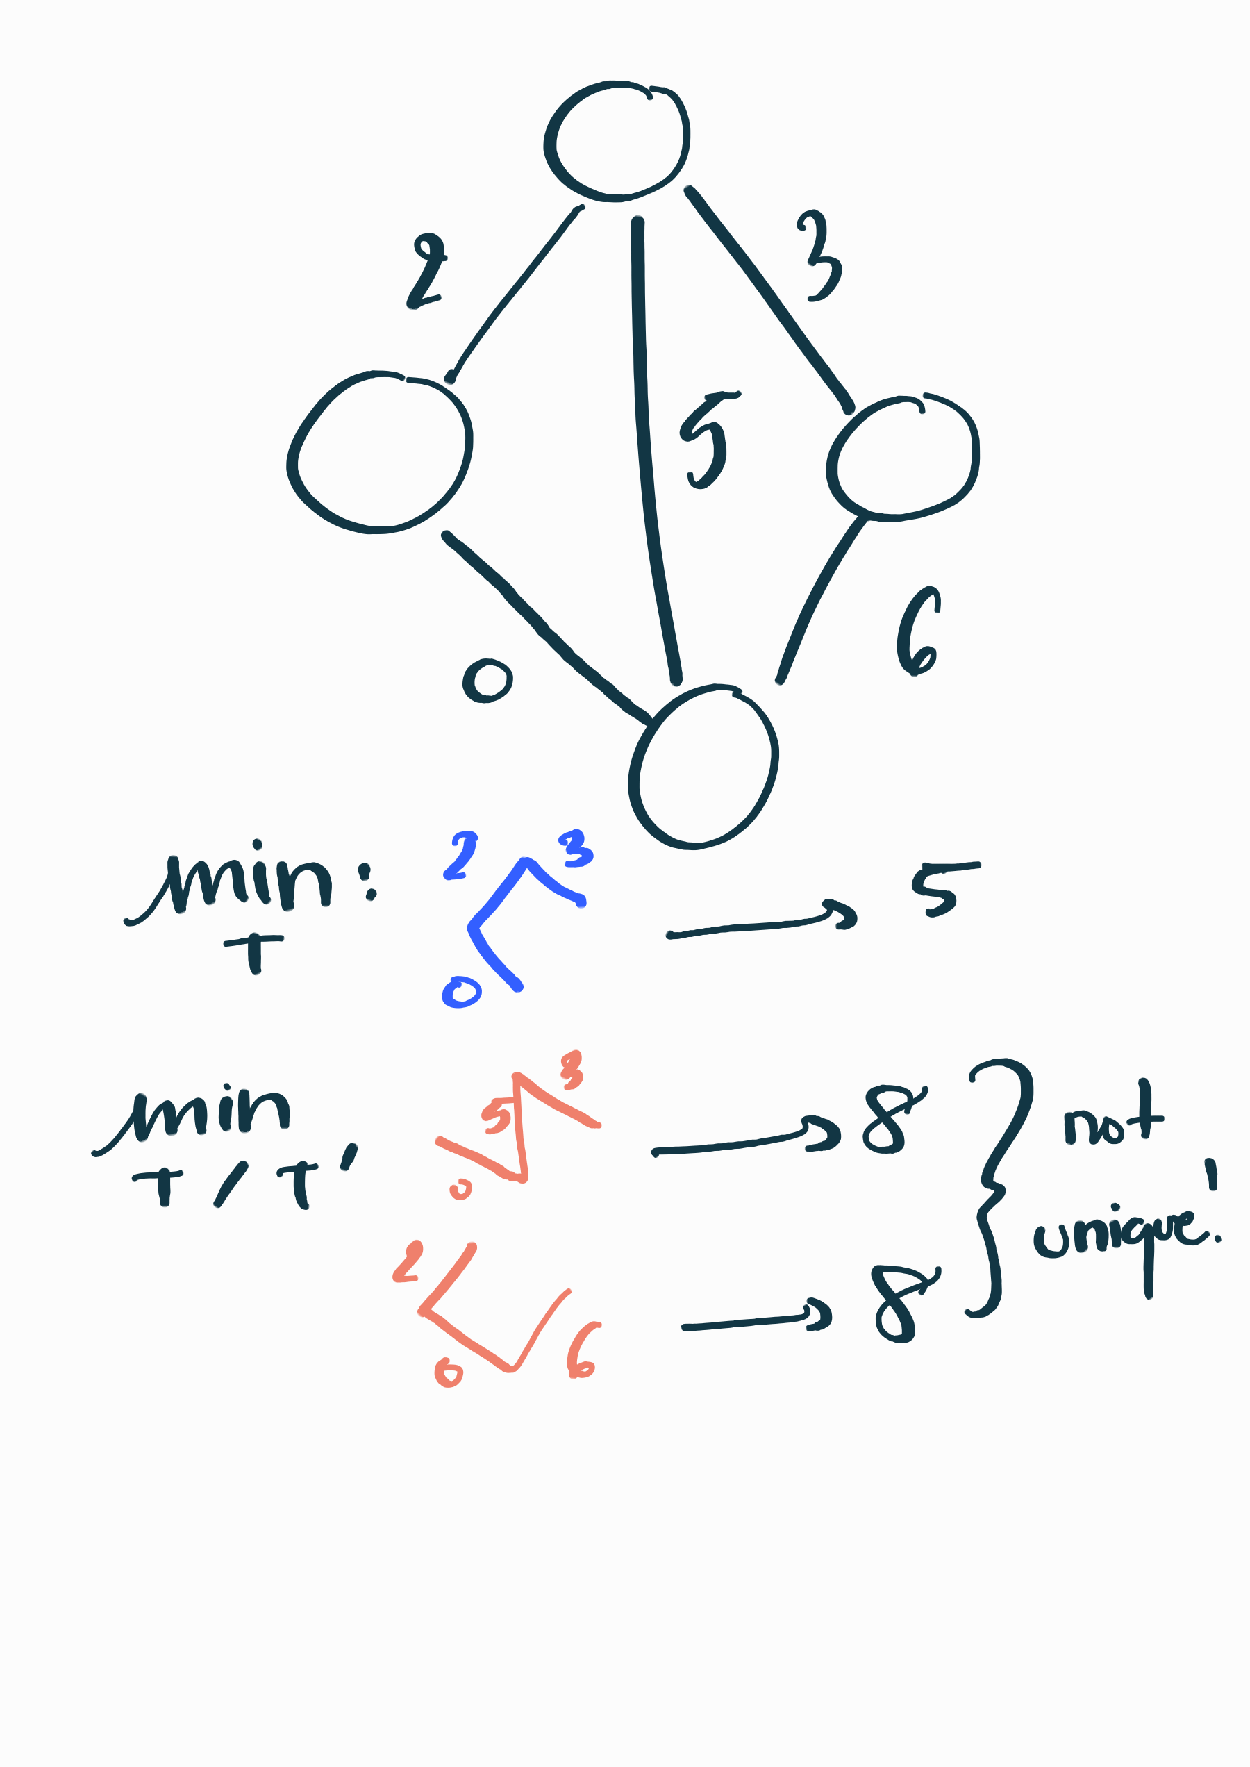
\includepdf[pages = {1}]{example.pdf}
\end{document}




